\chapter{Analýza}
Tato kapitola pojednává o analýze a návrhu vhodného řešení aplikace. Výstupem této analýzy jsou funkční a obecné požadavky. Dále návrh a popis domén a nejdůležitější případy užití s aktéry. 

\section{Požadavky}
Požadavky na systém se dělí na dvě sekce: obecné a funkční požadavky. Pro definování těchto požadavků jsem vycházel z oficiálního zadání práce tak i z prototypu aplikace, protože mi přesně definuje návrh aplikace a pro implementaci systému i potřebné technologie.

\subsection{Obecné požadavky}
Obecné požadavky se netýkají funkčnosti, ale celkového návrhu a použitých technologií.
\begin{enumerate}
\item Systém bude postaven na webovém frameworku Ruby on Rails.
\item Systém bude webovou aplikací.
\item Systém bude používat webovou službu KOSapi.
\item Systém bude pro autentizaci používat FELid.
\end{enumerate}

\subsection{Funkční požadavky}
Tato sekce se zabývá požadavky na funkčnost systému.
\begin{enumerate}
\item Systém umožní spravovat uživatele.
\item Systém umožní průběžné plánování hospitaci.
\item Systém umožní hospitujícímu i hospitovanému prohlížet hospitace \cite{prototyp_documentace}.
\item Systém umožní vystavit závěrečné hodnocení na veřejné části aplikace \cite{prototyp_documentace}. 
\item Systém umožní hospitovanému sepsat stanoviska k názorům hospitujícího \cite{prototyp_documentace}.
\item Systém umožní hospitujícímu nahrát naskenovaný dokument hodnocení výuky \cite{prototyp_documentace}.
\item Systém umožní hospitujícímu napsat slovní hodnocení z výuky \cite{prototyp_documentace}.
\item Systém umožní hospitujícímu napsat závěrečné shrnutí hospitace \cite{prototyp_documentace}.
\item Systém bude odesílat emailem zprávy o naplánování hospitací a jednotlivé hodnocení a stanoviska příslušným osobám \cite{prototyp_documentace}.
\item Systém umožní vyhledávat předměty z KOSapi.
\item Systém umožní vyhledávat osoby z KOSapi.
\item Systém umožní upravovat strukturu hodnotících dokumentů.
\end{enumerate}

\section{Uživatelské role}
V systému je celkem 6 uživatelských rolí, ty jsou odvozeny z modelu aktérů na obrázku \ref{fig:actors}. Máme tři základní uživatelské role, které jsou základem systému - přihlášený uživatel, nepřihlášený uživatel a administrátor hospitací. Další role, jako hospitovaný a hospitující uživatel, jsou přiděleny příslušným osobám zainteresovaných v jednotlivých hospitacích.

\begin{figure}[h]
\begin{center}
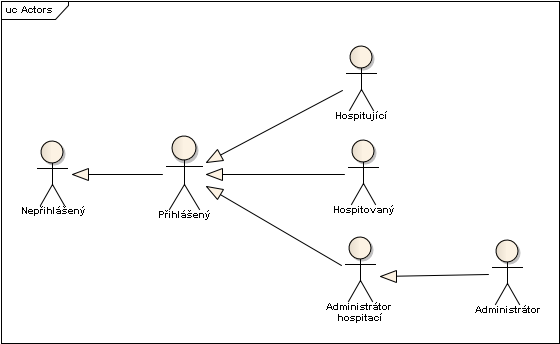
\includegraphics[width=14cm]{figures/Actors}
\caption{Aktéři}
\label{fig:actors}
\end{center}
\end{figure}

V systému jsou následující role:

\subsection{Nepřihlášený uživatel}
Nepřihlášený uživatel je role pro hosty naší aplikace. V systému má ze všech rolí nejmenší pravomoc. V tomto stavu je každý uživatel, který se doposud nepřihlásil do systému a je mu umožněno vykonat následující akce: přihlásit se, zobrazit seznam naplánovaných veřejných hospitací na aktuální a následující semestr, má také přístup k závěrečným shrnutím hospitací.

\subsection{Přihlášený uživatel}
Přihlášený uživatel vychází z role nepřihlášeného uživatele. Je to uživatel, který má vytvořený účet v systému a již se přihlásil. Tato role přidává možnost odhlásit se a procházet veškeré ohlášené hospitace. Jedná se o roli základní pro všechny další role, které z ní vychází.

\subsection{Hospitovaný}
Hospitovaný je role pro přihlášeného uživatele v systému. Je přidělena pro každého vyučujícího, který vyučuje předmět, na němž byla naplánovaná hospitace. Tato role přidává možnost přístupu k naplánovaným hospitacím, kde figuruje jako hospitovaný. U těchto hospitací má právo na zobrazení všech hodnotících dokumentů a umožní mu sepsat dokument se stanovisky k názorům hospitujícího.

\subsection{Hospitující}
Hospitující je role pro přihlášeného uživatele v systému. Přiděluje ji administrátor hospitací osobám, které mají za úkol vykonat hospitaci. U přidělených hospitací má uživatel právo na zobrazení informací o jeho hospitaci a povinnost sepsat hodnotící dokumenty z vykonané hospitace.

\subsection{Administrátor hospitací}
Tato role patří mezi nejdůležitější role v systému, protože spravuje hospitace a přiděluje uživatelům nové role. Hlavním úkolem této role je plánovat hospitace na předměty a posléze je spravovat.   

\subsection{Administrátor}
Administrátor je super uživatel, který má nejvyšší pravomoc v systému. Má přístup ke všem zdrojům aplikace a může nastavovat aplikaci.

\section{Doménový model}
Doménový model na obrázku \ref{fig:domainmodel} reprezentuje entity v systému a jejich vzájemné vztahy. 

Popis domény jsem pro přehlednost rozdělil podle zdroje na dvě základní skupiny. V první skupině jsou domény, které používám z KOSapi a druhou skupinou jsou domény specifické pro moji aplikaci. 

\subsection{Domény z KOSapi}
\begin{itemize}
\item Osoba - informace o osobě nacházející se na FEL. Každá osoba může být učitelem a studentem.
\item Semestr - informace o jednotlivých semestrech. 
\item Předmět - jednotlivé předměty vyučované na FEL.
\item Instance předmětu - jsou instance předmětu vypsané v konkrétním semestru.
\item Paralelka - je vypsaná rozvrhová paralelka pro instanci předmětu.
\item Místnost - informace o místech, kde probíhá výuka předmětů
\end{itemize}

\subsection{Domény aplikace}
\begin{itemize}
\item Uživatel - obsahuje dodatečné informace a role pro osobu v aplikaci.
\item Hospitace - obsahuje informace o naplánování hospitace. 
\item Poznámka - je textová poznámka pro hospitaci napsaná uživatelem.
\item Příloha - je připojený datový soubor k hodnocení hospitace.
\item Formulář - je vyplněný formulář pro hospitaci.
\item Hodnota - je vyplněná hodnota jedné formulářové položky.
\item Typ formuláře - udává formát dokumentu, který se používá pro hospitace. 
\item Položka - je šablona jedné položky ve formuláři.
\end{itemize}

\begin{figure}[h]
\begin{center}
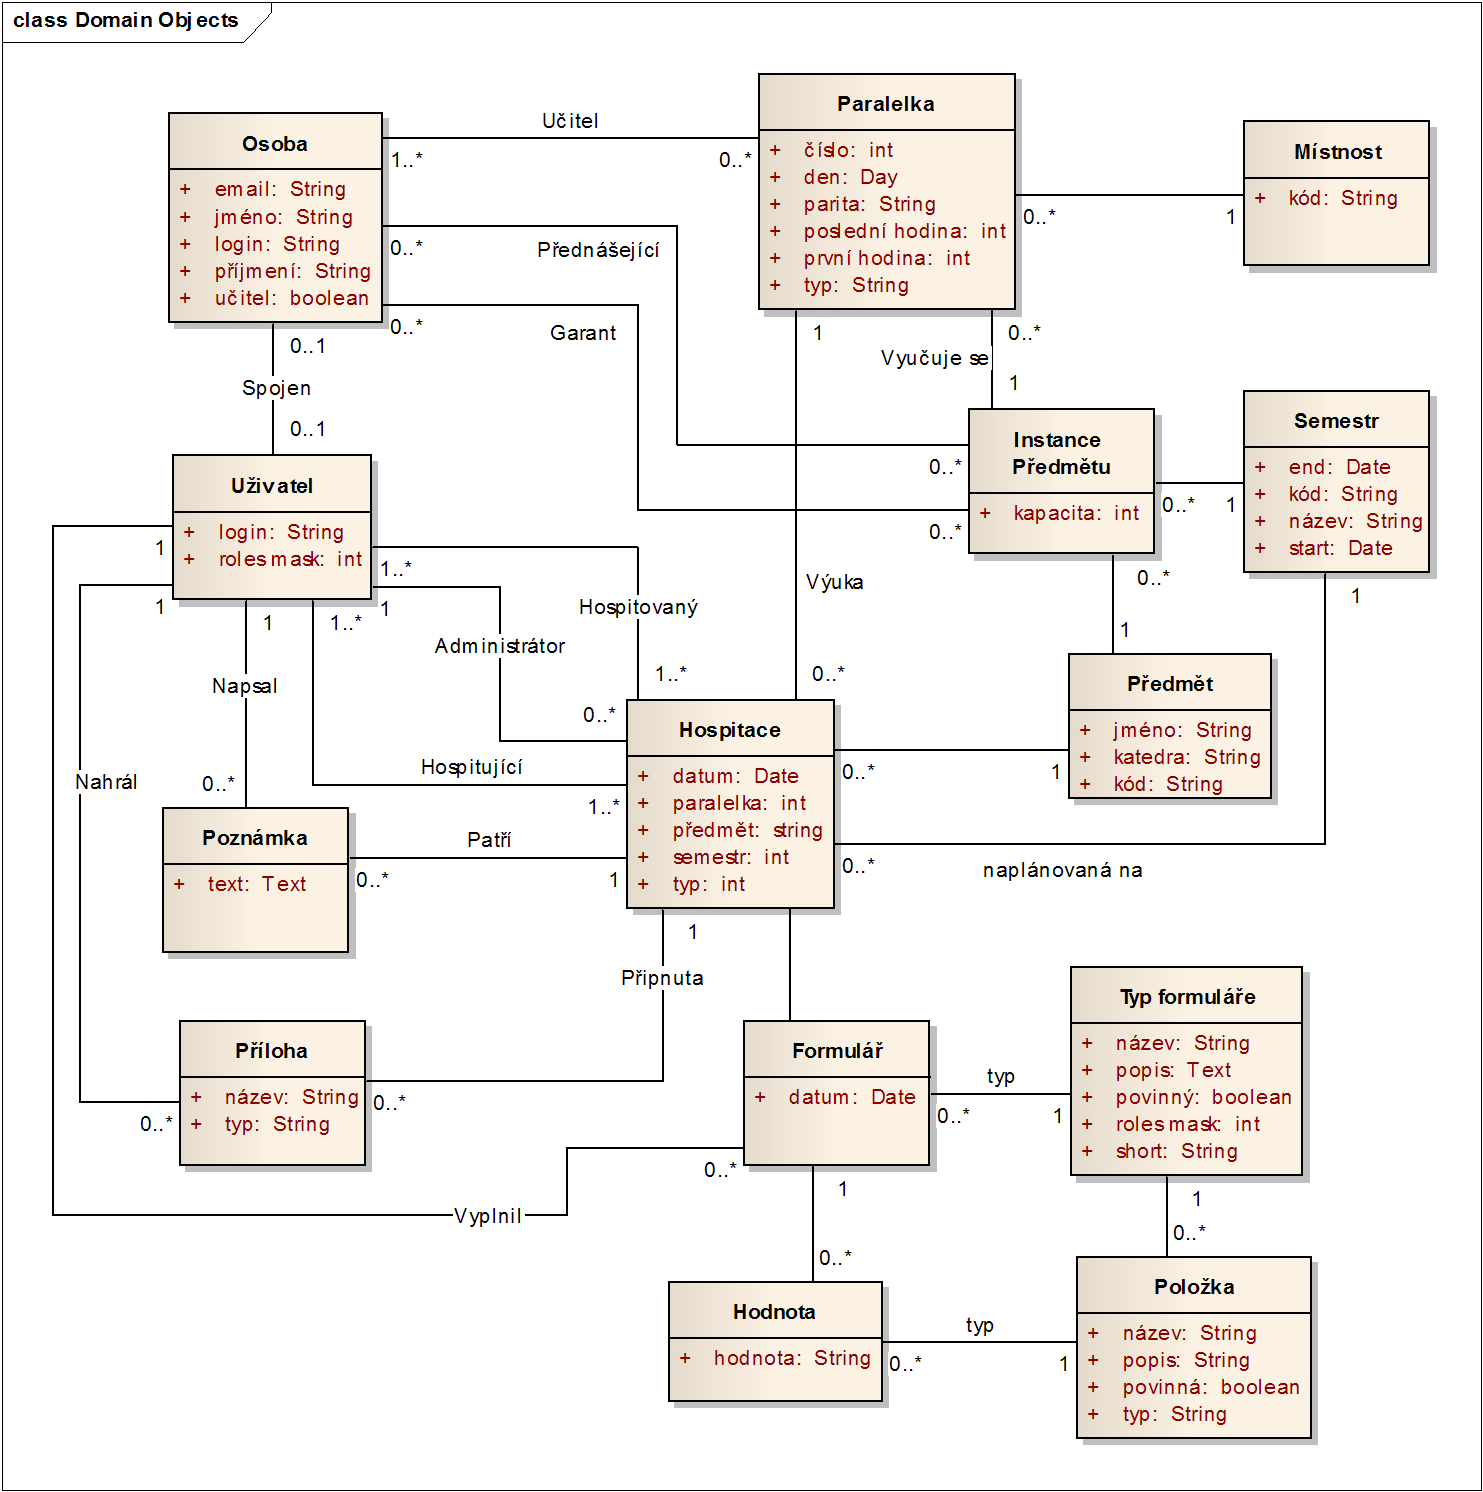
\includegraphics[width=14cm]{figures/DomainModel}
\caption{Doménový model}
\label{fig:domainmodel}
\end{center}
\end{figure}

\section{Životní cyklus hospitace}
Cílem této části analýzy je popsat životní cyklus, kterým hospitace prochází. 

\subsection{Vytvoření}
Životní cyklus hospitace začíná jejím vytvořením. Toto zajišťuje administrátor hospitací, který založí hospitaci a definuje semestr, kdy se má hospitace uskutečnit, a předmět vyučovaný na fakultě. Při vytváření hospitace se určí typ hospitace a tím i její způsob zviditelnění, pro ostatní aktéry v aplikaci.

\subsection{Naplánování}
Při plánování je také hlavním aktérem administrátor hospitace. V této části životního cyklu administrátor určí hospitovanou paralelku předmětu a datum,  kdy se hospitace uskuteční.  

Administrátor také v této fázi přidělí hospitující z řad pedagogů určených k vykonání hospitace.  
 
\subsection{Hodnocení}
Poté, co proběhla kontrola hospitace, začíná nová fáze, ve které se hodnotí vyučování. Do této fáze už nezasahuje administrátor hospitace, ale přicházejí na scénu dva jiní aktéři: hospitovaný a hospitující.

V první fázi musí hospitující vyplnit, nebo nahrát naskenovaný formulář pro Hodnocení výuky při hospitaci. Tento formulář slouží k dokumentaci průběhu hospitace.

V druhé fázi jeden z hospitujících sepíše slovní hodnocení hospitační návštěvy.

Ve třetí fázi může hospitovaný do dvou dnů vyplnit stanovisko hodnoceného k názorům hospitujícího.  

V poslední fázi jeden z hospitujících sepíše poslední formulář Závěrečné shrnutí. Po vyplnění tohoto formuláře se hospitace stává ukončenou a tím končí její životní cyklu.
 